\documentclass[dvipdfmx,tikz]{standalone}
\usepackage{tikz}
\usepackage{ifthen}


\usetikzlibrary{
  shapes,
  shapes.geometric,
  arrows.meta,
  calc,
}

\definecolor{cA}{HTML}{0072BD}
\definecolor{cB}{HTML}{EDB120}
\definecolor{cC}{HTML}{77AC30}
\definecolor{cD}{HTML}{D95319}

\begin{document}
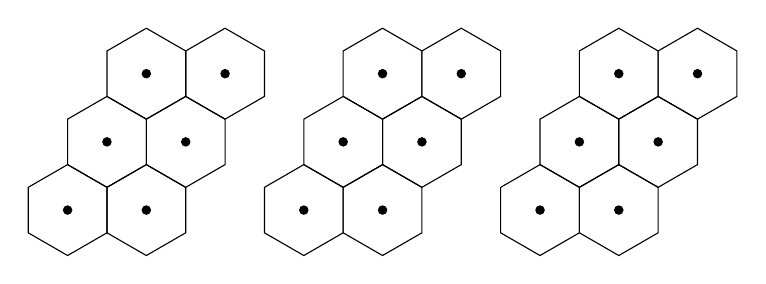
\begin{tikzpicture}
  \foreach \X in {0,1,2}{
      \begin{scope}[xshift=3*\X cm]
        \foreach \x in {0,1,2}{
            \foreach \y in {0,1}{
                \pgfmathsetmacro\shift{mod(\x,2)*0.5+max(\x-1,0)}
                \coordinate (a\x\y) at ({\y - \shift},{-sqrt(3)/2*\x});
              }}

        \foreach \x in {0,1,2}{
            \foreach \y in {0,1}{
                \filldraw[draw=black,fill=black] (a\x\y) circle (1.5pt);
                \node[regular polygon, regular polygon sides=6, minimum size=1.1547005cm, draw,rotate=30] at (a\x\y) {};
              }
          }
      \end{scope}
    }
\end{tikzpicture}
\end{document}
